\chapter{Uczenie maszyn}
Uczenie maszynowe jest dziedzina algorytmów komputerowych, które automatycznie poprawiają swoją efektywność poprzez doświadczenie. 
Określa się je jako poddziedzinę sztucznej inteligencji. Algorytmy te pozwalają na zbudowanie matematycznego modelu na podstawie 
przykładowych danych nazywanych danymi treningowymi co pozwala im na wykonywanie predykcji lub decyzji bez potrzeby ich dokładnego 
zaimplementowania przez programistę. Uczenie maszynowe stosuje się do wielu zadań jak filtrowanie poczty mailowej ze spamu, reklamy Internetowe, 
wykrywanie twarzy na zdjęciach oraz nagraniach a przyszłości może pomóc w stworzeniu takich technologii jak 
samojezdne samochody. Sam termin został spopularyzowany przez informatyka Arhura Samuela w roku 1959, był on autorem pierwszego działającego 
systemu tego typu, jego program automatycznie grał w warcaby i uczył się na podstawie poprzednich potyczek.
\section{Rodzaje}
\begin{figure}[h]
    \centering
    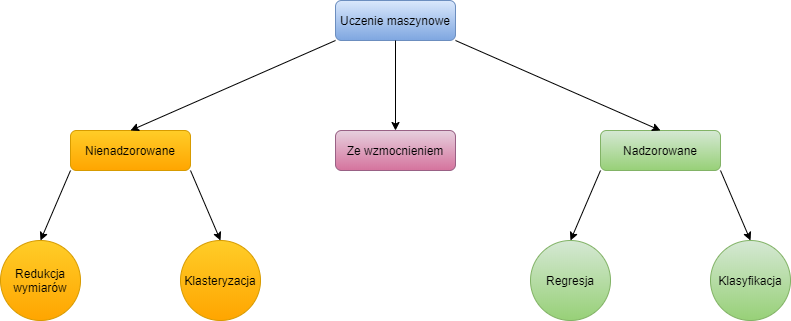
\includegraphics[width=1\textwidth]{./Img/typesofLearning.png}
    \caption{Rodzaje uczenia maszynowego Źródło: Własne}
\end{figure}
Algorytmy uczenia maszynowego można podzielić na trzy główne rodzaje w zależności od problemów, które mają one rozwiązywać są to:
\begin{enumerate}
    \item \textbf{Uczenie nadzorowane}
    Jest to najczęściej wykorzystywany rodzaj uczenia maszynowego polega on na tym 
    że maszyna uczy się na podstawie przykładów zawartych w danych treningowych 
    uczenie nadzorowane można porównać do nauczyciela i ucznia gdzie dane pełnią rolę nauczyciela 
    a program ucznia. Algorytmy tego typu potrafią znaleźć odpowiednie zależności na podstawie
    etykiet przypisanym danym,
    które następnie wykorzystują w celu predykcji wcześniej nie analizowanych danych.
    Ważnym zagadnieniem w przypadku uczenia nadzorowanego jest tak zwany Overfitting polegający 
    na przeuczeniu programu jednym zestawem treningowym przez co traci on umiejętność generalizacji problemu
    i nie jest w stanie poprawnie podejmować predykcji danych niewystarczająco podobnych
    do treningowych.

    Przykładowe zastosowanie:
    \begin{itemize}
        \item Klasyfikacja - przewidywanie kategorii
        \begin{itemize}
            \item rozpoznawanie elementów na zdjęciu
            \item filtrowanie spamu w skrzynce mailowej
        \end{itemize}
        \item Regresja - przewidywanie liczb
        \begin{itemize}
            \item przewidywanie trendów finansowych lub ekonomicznych,
            \item prognozowanie pogody
        \end{itemize}
    \end{itemize}
    \item \textbf{Uczenie nienadzorowane}
    W przeciwieństwie do uczenia nadzorowanego uczenie nienadzorowane opiera się na braku
    nauczyciela a zadaniem maszyny jest znalezienie wzorców i zależności między analizowanymi
    obiektami samodzielnie. Dwie metody które są najczęściej wykorzystywane w uczeniu nienadzorowanym
    to:
    \begin{enumerate}
        \item \textbf{Analiza składowych głownych} - Polega na zmniejszaniu wymiarowości danych poprzez
        odnajdywanie a następnie odrzucanie cech, które niosą ze sobą najmniejszą ilość informacji,
        \item \textbf{Analiza skupień (Klasteryzacja)} - Pozwala na identyfikację oraz grupowanie danych
        podobnych, które nie są w żaden sposób oznaczone. Może także pomóc w odnalezieniu anomalii
        nie pasujących do żadnej z wydzielonych grup.
        
    \end{enumerate} 
    Wykorzystanie tego typu algorytmów pozwala na badanie danych nieoznaczonych,
    które są znacznie częsciej spotykane niż dane oznaczone.
    
    Przykładowe zastosowanie:
    \begin{itemize}
        \item Redukcja wymiarów
        \begin{itemize}
            \item Wizualizacja danych ``big data''
            \item Kompresja danych
        \end{itemize}
        \item Klasteryzacja
        \begin{itemize}
            \item Spersonalizowane reklamy
            \item Systemy rekomendacyjne
        \end{itemize}
    \end{itemize}
    \item \textbf{Uczenie ze wzmocnieniem}
    Uczenie ze wzmocnieniem polega na wykorzystaniu metody prób i błędów w taki sposób by maszyna została
    ``nagrodzona'' za wykonywanie czynności pożądanych oraz ``karana'' za popełnianie błędów. 
    Sukces takiego systemu oparty jest na odpowiedniej implementacji systemu nagród, który może 
    mieć całkowicie inne działanie w zależności od rozwiązywanego problemu. 
    Ponieważ algorytmy uczenia ze wzmocnieniem dążą do zebrania jak największej
    ilości ``nagrody'' nie zawsze odnajdują one optymalne rozwiązanie.
    
    Przykładowe zastosowanie:
    \begin{itemize}
        \item Tworzenie programów grających w gry
        \item Samojezdne samochody
    \end{itemize}
\end{enumerate} 

\section{Algorytmy klasyfikacji}
Z problemem klasyfikacji można się spotkać wszędzie tam, gdzie wykorzystując
zbiór zmiennych objaśniających należy wskazać wartość przyjmowaną przez zmienną
modelowaną. W problemach klasyfikacji zmienna modelowana może przyjmować wartości
binarne (\textbf{klasyfikacja dwuklasowa}) lub jedną z wielu etykiet (\textbf{klasyfikacja wieloklasowa}).
Aby wybrać odpowiedni do rozwiązywanego problemu algorytm klasyfikacji należy wziąć 
pod uwagę 4 czynniki:
\begin{itemize}
    \item Złożoność czasowa - jak długo trwa uczenie oraz predykcja nowych danych,
    \item Interpretowalność - jak łatwo można wytłumaczyć decyzję podjętą przez 
    system,
    \item Skalowalność - jak dużą ilość zasobów zużywa dany algorytm,
    \item Czynnik ludzki - Aby poprawnie ustawić parametry algorytmu potrzebna
    jest wiedza na temat jego działania. Ponieważ poprawne ich ustawienie może 
    mieć większe znaczenie dla efektywności niż dobór najlepszego algorytmu często
    lepiej jest wykorzystać algorytm znany a nie optymalny.
\end{itemize}

\subsection{KNN}

Algorytm K najbliższych sąsiadów (\textbf{K nearest neighbours}) jest algorytmem
stosowanym zarówno w problemach regresyjnych jak i klasyfikacji. Kroki jego działania
można opisać w następujący sposób:
\begin{enumerate}
    \item Umieszczenie wszystkich obiektów posiadających N cech jako punkty w N-wymiarowej przestrzeni
    \item Obliczenie odległości między obiektem którego etykieta będzie przewidywana a każdym innym
    obiektem
    \item Przypisanie do obiektu etykiety, którą posiada większość z K najbliższych obiektów. 
\end{enumerate}
Faza uczenia w KNN polega wyłącznie na wczytaniu danych treningowych do pamięci przez co jest 
ona bardzo szybka.

Najważniejszą kwestią w poprawnym implementowaniu algorytmu KNN jest odpowiednie wybranie liczby
K, której optymalna wartość będzie się różnić w zależności od danych. W problemach 
klasyfikacji często wybiera się K o wartości nieparzystej aby uniknąć problemu remisu
podczas zliczania sąsiadów. W przypadku problemów regresyjnych zamiast wykonywać głosowanie
predykcję wykonuje się na podstawie średniej wartości K najbliższych sąsiadów.

\begin{table}[h]
    \begin{tabularx}{\linewidth}{>{\parskip1ex}X@{\kern4\tabcolsep}>{\parskip1ex}X}
    \toprule
    \hfil\bfseries Zalety
    &
    \hfil\bfseries Wady
    \\\cmidrule(r{3\tabcolsep}){1-1}\cmidrule(l{-\tabcolsep}){2-2}
    
    %% PROS, seperated by empty line or \par
    Prosty do zrozumienia i interpretacji\par
    Szybkość fazy uczenia\par
    Uniwersalność można go wykorzystać zarówno w problemach regresyjnych jak i klasyfikcyjnych\par
    Nie wykonuje generalizacji danych przez co jest efektywny w przypadku danych nieliniowych\par
    &
    
    %% CONS, seperated by empty line or \par
    Przechowuje wszystkie dane treningowe w pamięci co skutkuje wysoką złożonością pamięciową\par
    Wrażliwy na ilość danych i nieistotne cechy\par
    Kosztowny obliczeniowo\par
    \\\bottomrule
    \end{tabularx}
    \caption{Wady i zalety KNN}
\end{table}
    

\begin{figure}[h]
    \centering
    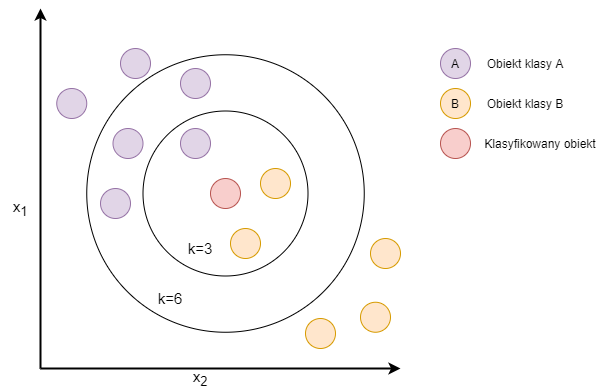
\includegraphics[width=0.8\textwidth]{./Img/KNN.png}
    \caption{Graficzne przedstawienie algorytmu KNN Źródło: Własne}
\end{figure}

\subsection{SVM}

Klasyfikator SVM (\textbf{Support vector machines}) również można wykorzystywać zarówno 
w problemach regresyjnych i klasyfikcyjnych. Służą one do klasyfikacji binarnej, co 
oznacza że obiekty należy podzielić na dokładnie dwie klasy. SVM polega na znalezieniu
takiej prostej lub płaszczyzny (w zależności od liczby cech), która w jak najlepszy sposób
dzieli obiekty dwóch klas. Czasami idealny podział jest niemożliwy z czym klasyfikator 
ten radzi sobie w jeden z dwóch sposobów:
\begin{enumerate}
    \item Ignorowanie punktów które uniemożliwiają podział,
    \item Wykorzystanie tak zwanych kernel trick, które przekształcają dane do wyższego 
    wymiaru w którym podział jest możliwy.
\end{enumerate}
Aby odnaleźć optymalne rozwiązanie SVM skupiają się na punktach jak najbardziej skrajnych
obu klas są one nazywane \textbf{wektorami nośnymi} zmiana ich położenia lub usunięcie
całkowicie zmienia położenie płaszczyzny.

\begin{table}[h]
    \begin{tabularx}{\linewidth}{>{\parskip1ex}X@{\kern4\tabcolsep}>{\parskip1ex}X}
    \toprule
    \hfil\bfseries Zalety
    &
    \hfil\bfseries Wady
    \\\cmidrule(r{3\tabcolsep}){1-1}\cmidrule(l{-\tabcolsep}){2-2}
    
    %% PROS, seperated by empty line or \par
    Efektywny w wielowymiarowych przestrzeniach\par
    Działa nawet w przypadku gdzie liczba danych treningowych jest mniejsza od
    ilości ich cech\par
    Przechowuje w pamięci tylko niewielką ilość danych treningowych\par
    
    &
    
    %% CONS, seperated by empty line or \par
    Nie jest on przystosowany do dużej ilości danych treningowych\par
    Nie radzi sobie dobrze jeżeli obiekty różnych klas nachodzą na siebie\par
    Trudne do zinterpretowania wyniki predykcji
    
    \\\bottomrule
    \end{tabularx}
    \caption{Wady i zalety SVM}
\end{table}

\begin{figure}[h]
    \centering
    \includegraphics[width=0.6\textwidth]{./Img/SVM.png}
    \caption{Wizualizacja algorytmu SVM Źródło: Własne}
\end{figure}

\subsection{MLP}

Działanie algorytmu Perceptronu wielowarstwowego (\textbf{Multi layered perceptron}) 
opiera się na wykorzystaniu modelu sztucznego neuronu, który na podstawie określonej
funkcji aktywacji oblicza na wyjściu pewną wartość na podstawie ważonych sum danych
wejściowych. 

Funkcje aktywacji dzieli się na:
\begin{itemize}
    \item \textbf{Funkcje progowe} z wyjściem binarnym
    \item \textbf{Funkcje liniowe} z wyjściem ciągłym
    \item \textbf{Funkcje nieliniowe} z wyjściem ciągłym
\end{itemize}
W sieciach wielowarstwowych najczęściej wykorzystuje się funkcje nieliniowe poniważ 
wykazują one najwieksze zdolności do nauki.

Perceptron wielowarstwowy składa się z trzech warstw sztucznych neuronów: 
\begin{enumerate}
    \item \textbf{Warstwy wejściowej} - są to neurony zapewniające całej sieci
    informacje czyli zazwyczaj dane treningowe nie wykonują one żadnych obliczeń
    a jedynie przekazują informacje do kolejnych warstw.
    \item \textbf{Warstwy ukrytej} - wykonują one odpowiednie obliczenia zmieniając 
    i przekazując informacje z warstwy wejściowej do wyjściowej. Sieć może składać
    się z dowolnej liczby warstw ukrytych.
    \item \textbf{Warstwy wyjsćiowej} - wykonują one ostatnie obliczenia na danych 
    a następnie zwracają wynik.
\end{enumerate}

Uczenie takiej sieci polega na takiej modyfikacji wag na wejściu neuronów aby poprawić
wyniki klasyfikacji. Podczas gdy perceptron jednowarstwowy czyli nieposiadający żadnej warstwy ukrytej może 
nauczyć się wyłącznie funkcji liniowych perceptron wielowarstwowy pozwala na nauczenie
się skomplikowanych funkcji nieliniowych.

\begin{table}[h]
    \begin{tabularx}{\linewidth}{>{\parskip1ex}X@{\kern4\tabcolsep}>{\parskip1ex}X}
    \toprule
    \hfil\bfseries Zalety
    &
    \hfil\bfseries Wady
    \\\cmidrule(r{3\tabcolsep}){1-1}\cmidrule(l{-\tabcolsep}){2-2}
    
    %% PROS, seperated by empty line or \par
    Szybkie wykonywanie predykcji po nauczeniu modelu\par
    Efektywny dla nieliniowych danych posiadających wiele cech takich jak zdjęcia\par
    Działają najlepiej dla dużej ilości danych treningowych\par
    &
    
    %% CONS, seperated by empty line or \par
    Brak możliwości interpretacji wyniku predykcji\par
    Uczenie bardzo złożone obliczeniowo co skutkuje długim czasem uczenia\par
    Użytkownik ma niewielki wpływ na działanie sieci\par
    \\\bottomrule
    \end{tabularx}
    \caption{Wady i zalety MLP}
\end{table}

\begin{figure}[h]
    \centering
    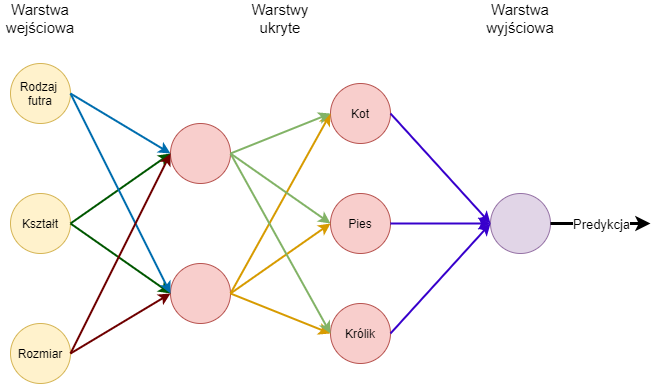
\includegraphics[width=0.8\textwidth]{./Img/MLP.png}
    \caption{Graficzne przedstawienie perceptronu wielowarstwowego Źródło: Własne}
\end{figure}

\subsection{Decision trees}

Algorytm Decision trees polega na stworzeniu drzewa decyzyjnego w którym korzeń i węzły
są poszczególnymi cechami zbioru danych a liście odpowiadają klasom, które tym danym 
należy przypisać, ostatnim elementem są krawędzie którymi reprezentuje się wartości cech. 
Kroki algorytmu są następujące:
\begin{enumerate}
    \item Wybranie najlepszej cechy
    \item Dodanie gałęzi odpowiadającym poszeczególnym wartościom wybranej cechy
    \item Podział zbioru danych na podzbiory zgodnie z wartościami cechy
    \item Jeżeli wszystkie elementy pozdzbiorów należą do tej samej klasy 
    zakończenie gałęzi liściem. W przeciwnym wypadku powtórzenie kroków 
    od 1 do 4 dla każdego podzbioru
\end{enumerate}
Aby dokonać optymalnego podziału algorytm musi wybrać cechy powodujące jak najlepsze
podzielenie różnych klas a więc niosące ze sobą największą ilośc informacji,
wykorzystuje się w tym celu entropię, której wartość pozwala określić średnią ilość 
informacji niesioną przez poszczególne cechy.
\begin{equation}
    H(x)=-\sum_{i=1}^n p(x_i) \log_2 p(x_i).
    \label{eq-entropy}
\end{equation}
Wzór na entropię ~\ref{eq-entropy}, gdzie \textit{p(x\textsubscript{i})} jest prawdopodobieństwem
wybrania klasy \textit{x\textsubscript{i}}
\begin{table}[h]
    \begin{tabularx}{\linewidth}{>{\parskip1ex}X@{\kern4\tabcolsep}>{\parskip1ex}X}
    \toprule
    \hfil\bfseries Zalety
    &
    \hfil\bfseries Wady
    \\\cmidrule(r{3\tabcolsep}){1-1}\cmidrule(l{-\tabcolsep}){2-2}
    
    %% PROS, seperated by empty line or \par
    Łatwe do zinterpretowania wyniki bardzo wygodne do zwizualizowania\par
    Automatyczna selekcja ważnych cech. Obecność cech zbędnych nie ma wpływu na efektywność\par
    Szybkie wykonywanie predykcji\par
    &
    
    %% CONS, seperated by empty line or \par
    Wrażliwy na przeuczenie\par
    Potrzeba stworzenia nowego drzewa podczas dodawania nowych danych\par
    Małe zmiany w danych treningowych maja duży wpływ na predykcję\par
    
    \\\bottomrule
    \end{tabularx}
    \caption{Wady i zalety Drzew decyzyjnych}
\end{table}

\begin{figure}[h]
    \centering
    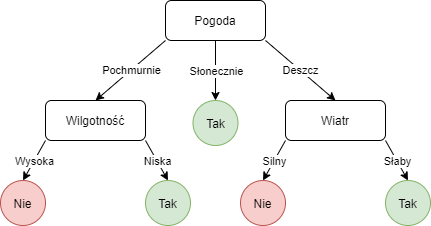
\includegraphics[width=0.8\textwidth]{./Img/BinaryTree.png}
    \caption{Przykładowe drzewo decyzyjne podejmujące decyzję czy wyjść na zewnątrz Źródło: Własne}
\end{figure}


\subsection{Naive Bayes}

Naiwny klasyfikator Bayesowski (\textbf{Naive Bayes}) jest probabilistycznym klasyfikatorem, który
zakłada wzajemną niezależność wszystkich cech stąd naiwność algorytmu. Stworzony przez niego model
opiera się na obliczeniu prawdopodobieństw wystąpienia poszczególnych cech pod warunkiem że 
występują one w danej klasie. Pozwala to przy użyciu twierdzenia Bayesa ~\ref{eq:bayes} obliczyć prawdopodobieństwa 
warunkowe określające z jak duża pewnością występująca kombinacja cech prowadzi do 
wystąpienia róznych klas na podstawie czego algorytm wykonuje predykcję. 


\begin{equation}
    \label{eq:bayes}
    P(A|B) = \frac{P(A|B)P(A)}{P(B)}
\end{equation}
gdzie P(A) i P(B) prawdopodobieństwa wystąpienia zdarzeń A i B, P(A|B) prawdopodieństwo wystąpienia
zdarzenia A pod warunkiem wystąpienia zdarzenia B.

Algorytm ten jest często wykorzystywany w systemach czasu rzeczywistego, ponieważ działa bardzo szybko 
kosztem efektywności.
\begin{table}[h]
    \begin{tabularx}{\linewidth}{>{\parskip1ex}X@{\kern4\tabcolsep}>{\parskip1ex}X}
    \toprule
    \hfil\bfseries Zalety
    &
    \hfil\bfseries Wady
    \\\cmidrule(r{3\tabcolsep}){1-1}\cmidrule(l{-\tabcolsep}){2-2}
    
    %% PROS, seperated by empty line or \par
    Bardzo szybki nawet w przypadku przewidywania wieloklasowego\par
    Działa nawet dla małej ilości danych\par
    Dobra efektywność w przypadku klasyfikacji danych wielowymiarowych
    jak na przykład w przypadku klasyfikacji tekstu\par
    
    &
    
    %% CONS, seperated by empty line or \par
    Jeżeli pewna cecha nie pojawi się w danych treningowych a istnieje w danych 
    testowych algorytm nie będzie w stanie wykonać jego predykcji\par
    Przyjmuje niezależność cech co w rzeczywistości jest prawie niespotykane\par
    Mniejsza efektywność w porównaniu z bardziej skomplikowanymi algorytmami\par
    
    \\\bottomrule
    \end{tabularx}
    \caption{Wady i zalety Naive Bayes}
\end{table}

\section{Zagrożenia}
